\providecommand{\main}{../..}
\documentclass[\main/notes.tex]{subfiles}

\begin{document}
	\setcounter{chapter}{5}
	\chapter{Computer Networks}
		\section{Telecommunications}
			\begin{definition}{Telecommunications}
				The electronic transmission of signals for communication; enables organisations to carry out their processes and tasks through effective computer networks.
			\end{definition}
			\begin{description}[nosep]
				\item[1. Sending Unit] A person, computer system, terminal, or other device, that originates a message.
				\item[2. Signal] Transmitted by sending unit.
				\item[3. Telecommunications Device] Hardware component that facilitates electronic communication.
				\item[4. Medium] Any material substance that carries an electronic signal to support communications between a sending and receiving device.
				\item[5. Another Telecommunications Device]
				\item[6. Receiving Unit] 
			\end{description}
			\begin{center}
				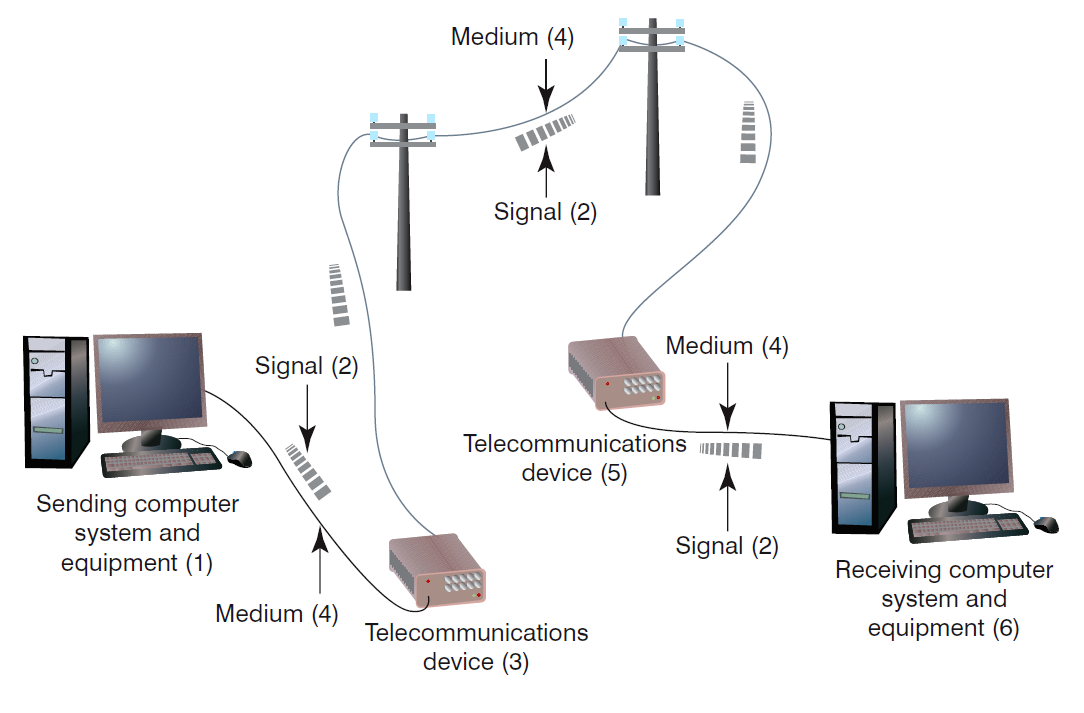
\includegraphics[width=0.75\textwidth]{chapter06/telecommunications_system.png}
			\end{center}
			The speed at which information is transmitted is measured in bits per second (bps), and typically range from thousands (Kbps) to millions (Mbps) to billions (Gbps).
			\begin{sidenote}{Synchronous vs Asynchronous}
				\begin{description}[nosep]
					\item[Synchronous] The receiver gets the message almost instantaneously when it is sent. For example, phone communication.
					\item[Asynchronous] There is a measurable delay between the sending and receiving of the message. For example, sending a message through the post office or via email.
				\end{description}
			\end{sidenote}
			\begin{definition}{Channel Bandwidth}
				The rate at which data is exchanged over a communications channel, usually measured in bits per second.

				The broader the bandwidth, the more information can be exchanged at one time.
				\begin{description}[nosep]
					\item[Broadband communications] A telecommunications system in which a very high rate of data exchange is possible.
					\item[Narrowband communications] A telecommunications system that supports a much lower rate of data exchange than broadband.
				\end{description}
			\end{definition}
			Transmission media can be divided into two types:
			\begin{indentparagraph}
				\begin{description}[nosep]
					\item[Guided Transmission Media] Communication signals are guided along a solid medium
					\item[Wireless Transmission Media] Communication signals are broadcast over airwaves as a form of electromagnetic radiation. 
				\end{description}
			\end{indentparagraph}
			\subsection{Guided Transmission Media Types}
				\begin{sidenote}{Guided Media Types}
					\begin{center}
						\begin{tblr}{colspec={>{\raggedright}X[2]>{\raggedright}X[3]>{\raggedright}X[3]>{\raggedright}X[3]}, row{even}={white}, row{1}={font=\bfseries}, column{1}={font=\bfseries}}
							Media Types & Description & Advantages & Disadvantages\\
							\midrule
							Twisted-pair wire & Twisted pairs of copper wires, shielded or unshielded & Used for telephone service; widely available & Transmission speed and distance limitations\\
							Coaxial Cable & Inner conductor wire surrounded by insulation & Cleaner and faster data transmission than twisted-pair wire & More expensive than twisted-pair wire\\
							Fibre-optic cable & Many extremely thin strands of glass bound together in a sheathing; uses light beams to transmit signals & Diameter of cable is much smaller than coaxial; less distortion of signal; capable of high transmission rates & Expensive to purchase and install\\
							Broadband over power lines & Data is transmitted over standard high-voltage power lines & Can provide Internet service to rural areas where cable and phone service may be non-existent & Can be expensive, and may interfere with amateur radios, police and fire communications 
						\end{tblr}
					\end{center}
				\end{sidenote}
			\subsection{Wireless Transmission Media Types}
				\subsubsection{Microwave Transmission}
					\begin{definition}{Microwave Transmission}
						High frequency (300 MHz to 300 GHz) signal sent through the air. Terrestrial (earth-bound) microwaves are transmitted by \concept{line-of-sight devices}. Can carry thousands of channels at the same time.
					\end{definition}
					\begin{sidenote}{Communications Satellites}
						A communications satellite also operates in the microwave frequency range. The advantage is that is can receive and broadcast over large geographic regions.
						\begin{description}
							\item[Geostationary Satellite] Orbits the Earth directly over the Equator, positioned a large distance above the Earth, so that it appears stationery. Three such satellites, spaced at even intervals, can span the entire Earth. Can be accessed using a dish antenna aimed at the spot in the sky where the satellite hovers.
							\item[Low Earth Orbit Satellite (LEO)] Employs many satellites, each in a circular orbit at an altitude of a few hundred kilometres.
							\item[Very Small Aperture Terminal (VSAT)] A two-way satellite ground station with a dish antenna smaller than three metres in diameter.
						\end{description}
					\end{sidenote}
				\subsubsection{5G Wireless Communication}
					\begin{sidenote}{Wireless Communication Generations}
						\begin{description}
							\item[First Generation (1G)] Originated in the 1980s, based on analogue communications.
							\item[Second Generation (2G)] Early 1990s, fully digital. Phone conversations encrypted, mobile phone usage expanded, \concept{short message services (SMS)} introduced.
							\item[Third Generation (3G)] Supports wireless voice and broadband speed data communications in a mobile environment at speeds of 2 to 4 Mbps. Mobile video, mobile e-commerce, location-based services, mobile gaming, downloading and playing music.
							\item[Fourth Generation (4G)] More advanced versions of enhanced multimedia, smooth streaming video, universal access and portability. 20 times the speed of 3G.
							\item[Fifth Generation (5G)] Higher data transmission rates, lower power consumption, higher connection reliability, increased geographic coverage, lower infrastructure costs. 
						\end{description}
					\end{sidenote}
				\subsubsection{Wi-Fi}
					\begin{definition}{Wi-Fi}
						A medium-range wireless telecommunications technology brand owned by the Wi-Fi alliance.

						The user's device has a wireless adapter that translates data into a radio signal and transmits it using an antenna. A \concept{wireless access point}, which consists of a transmitter with an antenna, receives the signal and decodes it.
					\end{definition}
				\subsubsection{Near Field Communication}
					\begin{definition}{Near Field Communication (NFC)}
						A very short-range wireless connectivity technology designed for credit cards, consumer electronics, and smartphones.

						Works with 2 devices, that need to be in proximity (touching, or a few centimetres apart). Exchange the necessary communications parameters to enable Bluetooth, Wi-Fi, or other communications between the devices. Establishes a \concept{peer-to-peer network}.
					\end{definition}
				\subsubsection{Bluetooth}
					\begin{definition}{Bluetooth}
						A wireless communication specification that describes how smartphones, computers, printers, and other devices can be interconnected over distances of a few meters at a rate of about 2 Mbps.
					\end{definition}
				\subsubsection{Ultra Wideband}
					\begin{definition}{Ultra Wideband (UWB)}
						A form of short-range communication that employs extremely short electromagnetic pulses lasting 50 to 1000 picoseconds that are transmitted over a broad range of radio frequencies or several gigahertz.

						Advantages: A high throughput rate, the ability to transmit undetected, and impervious to interception or jamming, and a lack of interference with current communications services.
					\end{definition}
				\subsubsection{Infrared Transmission}
					\begin{definition}{Infrared Transmission (IR)}
						A mode of transmission that sends signals through the air via light waves at a frequency of 300 GHz and above. Requires line-of-sign transmission, and short distances.
					\end{definition}
			\pagebreak
			\subsection{Telecommunications Hardware}
				\subsubsection{Modems}
					\begin{definition}{Analogue Signal}
						A variable signal continuous in both time and amplitude, so that any small fluctuations in the signal are meaningful.
					\end{definition}
					\begin{definition}{Digital Signal}
						A signal that represents bits.
					\end{definition}
					\begin{definition}{Modem (Modulator/Demodulator)}
						A telecommunications hardware device that modulates and demodulates communications signals, so they can be transmitted over the communication media.
						\begin{description}
							\item[Modulation] Translating data from digital to analogue.
							\item[Demodulation] Translating data from analogue to digital. 
						\end{description}
					\end{definition}
				\subsubsection{Multiplexers}
					\begin{definition}{Multiplexer}
						A device that encodes data from two or more data sources onto a single communications channel, this reducing their number of communications channels needed and therefore lowering telecommunications costs.
					\end{definition}
				\subsubsection{Front-End Processors}
					\begin{definition}{Front-End Processor}
						A special-purpose computer that managers communications to and from a computer system serving hundreds or even thousands of users.
					\end{definition}
				\subsubsection{Private Branch Exchange}
					\begin{definition}{Private Branch Exchange (PBX)}
						A telephone switching exchange that serves a single organisation.

						Enables users to share a certain number of outside lines (\concept{trunk lines}) to make telephone calls to people outside the organisation.
					\end{definition}
				\subsubsection{Switches, Bridges, Routers, and Gateways}
					\begin{definition}{Switch}
						A telecommunications device that uses the physical device address in each incoming message on the network, to determine to which output port it should forward the message, to reach another device on the same network.
					\end{definition}
					\begin{definition}{Bridge}
						A telecommunications device that connects one LAN to another LAN that uses the same telecommunications protocol.
					\end{definition}
					\begin{definition}{Router}
						A telecommunications device that forwards data packets across two or more distinct networks towards their destinations, through a process known as \concept{routing}.
					\end{definition}
					\begin{definition}{Gateway}
						A telecommunications device that serves as an entrance to another network.
					\end{definition}

		\section{Networks and Distributed Processing}
			\begin{definition}{Computer Network}
				The communications media, devices, and software needed to connect two or more computer systems or devices.
				\begin{description}
					\item[Network Nodes] The computers and devices on the network.
				\end{description}
			\end{definition}
			\subsection{Network Types}
				\begin{definition}{Personal Area Network (PAN)}
					A network that supports the interconnection of information technology within a range of ten metres or so.

					One device serves as the controller during wireless PAN initialisation, and this controller device mediates communication within the PAN.

					The Bluetooth communication protocol is the industry standard for PAN communications.
				\end{definition}
				\pagebreak
				\begin{definition}{Local Area Network (LAN)}
					A network that connects computer systems and devices within a small area, such as an office, home, or several floors in a building.

					Often use twisted-pair wire, but other media, such as fibre-optic cable, is also popular.

					A basic type of LAN is a simple peer-to-peer network that a small business might use to share files and hardware devices, such as printers.
					\begin{description}
						\item[Peer-to-peer network] A network where each computer is set up as an independent computer, but other computers can access specific files on its hard drive, or share its printer. The networks have no server. 
					\end{description}
				\end{definition}
				\begin{definition}{Metropolitan Area Network (MAN)}
					A telecommunications network that connects users and their devices in a geographical area that spans a campus or city.

					Most MANs have a range of roughly 100 kilometres.
				\end{definition}
				\begin{definition}{Wide Area Network (WAN)}
					A telecommunications network that ties together large geographic regions.
				\end{definition}
				\begin{definition}{Mesh Networking}
					A way to route communications between network nodes, by allowing continuous connections and reconfiguration around blocked paths, and `hopping' from node to node, until a connection can be established.
					\begin{description}
						\item[Full Mesh Topology] Each node is connected directly to each of the other nodes.
						\item[Partial Mesh Topology] Some nodes might be connected to all the others, and other nodes are connected only to nodes with which they frequently exchange information.
					\end{description}
					Robust -- if one node fails, all the other nodes can still communicate with each other, directly or through one of more intermediate nodes.
				\end{definition}
			\subsection{Distributed Processing}
				\begin{definition}{Centralised Processing}
					A processing alternative in which all processing occurs at a single location or facility.

					Offers the highest degree of control, as a single centrally managed computer performs all data processing.
				\end{definition}
				\pagebreak
				\begin{definition}{Decentralised Processing}
					A processing alternative in which processing devices are placed at various remote locations.

					Each computer system is isolated, and does not communicate with another system. Suitable for companies with independent operating divisions.
				\end{definition}
				\begin{definition}{Distributed Processing}
					A processing alternative where computers are placed at remote locations, but connected to each other via telecommunications devices.

					A benefit is that managers can allocate data to the locations that can process it most efficiently.
				\end{definition}
			\subsection{Client/Server Systems}
				\begin{definition}{Client/Server Architecture}
					An architecture in which multiple computer platforms are dedicated to special functions, such as database management, printing, communications, and program execution.
					\begin{description}
						\item[Server] One of these computer platforms that is dedicated to a special function. Accessible by all computers on the network.
							\begin{description}
								\item[Application server] Holds the programs and data for a particular application.
								\item[Email server] Sends and receives emails.
								\item[Web server] Sends out web pages.
							\end{description}
						\item[Client] Any computer that sends messages requesting services from the servers on the network.
					\end{description}
				\end{definition}
			\subsection{Communications Software}
				\begin{definition}{Network Operating System (NOS)}
					Systems software that controls the computer systems and devices on a network, and allows them to communicate with each other.

					Performs the same types of functions for the network as operating system software does for a computer.
				\end{definition}
				\pagebreak
				\begin{definition}{Network-Management Software}
					Software that enables a manager on a networked desktop to monitor the use of individual computers and shared hardware, scan for viruses, and ensure compliance with software licences.

					Simplifies the process of updating files and programs on computers on the network. Protects software from being copied, modified, or downloaded illegally.

					\concept{Fault detection} and \concept{performance management} are the two types of network-management produces. Both employ the \concept{Simple Network Management Protocol (SNMP)} to obtain key information from individual network components.
					\begin{description}
						\item[Fault Management Software] Alerts IS staff in real time when a device is failing.
						\item[Performance Management Software] Sends messages to the various devices, to sample their performance and to determine whether they are operating within acceptable levels.
					\end{description}
				\end{definition}
			\subsection{Software-Defined Networking}
				\begin{definition}{Software-Defined Networking (SDN)}
					An emerging approach to networking, that allows network administrators to manage a network via a controller that does not require physical access to all the network devices.

					SDN automates tasks such as configuration and policy management, and enables the network to dynamically respond to application requirements.
				\end{definition}
			\subsection{Securing Data Transmission}
				\begin{definition}{Encryption}
					The process of converting an original message into a form that can be understood only by the intended receiver.
					\begin{description}
						\item[Encryption Key] A variable that is applied (using an algorithm) to a set of unencrypted text to produce encrypted text, or to decrypt encrypted text. 
					\end{description}
					Encryption relies on the limitation of computing power for their security.
				\end{definition}
				\subsubsection{Securing Wireless Networks}
					\begin{definition}{Wired Equivalent Privacy (WEP)}
						Used to use an encryption based on 64-bit keys, now upgraded to 128-bit keys. An early attempt at securing wireless communications, and is not difficult for hackers to crack.
					\end{definition}
					\begin{definition}{Wi-Fi Protected Access (WPA)}
						A security protocol that offers significantly improved protection over WEP.
					\end{definition}
					\begin{sidenote}{Steps to safeguard a wireless network}
						\begin{itemize}
							\item Connect to the router and change the default login and password for the router
							\item Create a \concept{service set identifier (SSID)}, a 32-character unique identifier attached to the header portion of packets sent over a wireless network that differentiates one network from another.
							\item Configure the security to WPA
							\item Disable SSID broadcasting
						\end{itemize}
					\end{sidenote}
			\subsection{Virtual Private Networks}
				\begin{definition}{Virtual Private Network (VPN)}
					A private network that uses a public network (usually the Internet) to connect multiple remote locations.

					Provides network connectivity over a potentially long physical distance, and can be considered a form of wide area network.
				\end{definition}

		\section{The Internet}
			\begin{definition}{The Internet}
				The world's largest computer network -- a collection of interconnected networks, all freely exchanging information.
			\end{definition}
			\begin{definition}{ARPANET}
				A project started by the US Department of Defense (DoD) in 1969, as both an experiment in reliable networking, and a means to link DoD and military research contractors, including many universities doing military-funded research
			\end{definition}
			\begin{definition}{Internet Protocol (IP)}
				A communication standard that enables traffic to be routed from one network to another as needed. The set of conventions used to pass packets from one host to another.
			\end{definition}
			\subsection{How the Internet Works}
				The Internet transmits data from one computer (called a \concept{host}) to another. The various networks that are linked to form the Internet pass data around in chunks called \concept{packets}, each of which carries the addresses of its sender and its receiver.
				\begin{definition}{Transmission Control Protocol (TCP)}
					The widely used transport-layer protocol that most Internet applications use with IP.
				\end{definition}
				\begin{definition}{Backbone}
					One of the Internet's high-speed, long-distance communications links.
				\end{definition}
				\begin{definition}{Uniform Resource Locator (URL)}
					An assigned address on the Internet for each computer. Used to identify the computer to other hosts.
					\begin{example}
						Given the URL: \texttt{http://www.cengage.co.uk}
						\begin{description}
							\item[\texttt{http://}] The access method to use. In this case, \concept{Hypertext Transport Protocol}. The primary method for interacting with the Internet.
							\item[\texttt{www}] The files associated with the website reside on the \concept{World Wide Web server}.
							\item[\texttt{cengage.co.uk}] The domain name that identifies the Internet host site.
								\begin{description}
									\item[\texttt{cengage}] The name of the website (host network, or host provider).
									\item[\texttt{co.uk}] The \concept{top-level domain (TLD)}.
								\end{description}
						\end{description}
					\end{example}
				\end{definition}
				\begin{definition}{Internet Service Provider (ISP)}
					Any company that provides people of organisations with access to the Internet.
				\end{definition}

		\section{Internet Applications}
			\subsection{The World Wide Web}
				\begin{definition}{World Wide Web (WWW or W3)}
					A collection of tens of thousands of independently owned computers that work together as one in an Internet service. These computers are called \concept{web servers}.

					The web is a menu-based system that uses the client/server model. It organises Internet resources throughout the world into a series of menu pages or screens that appear to your computer. 
				\end{definition}
				\begin{definition}{Home Page}
					A cover page for a website, that has graphics, titles, and text.
				\end{definition}
				\begin{definition}{Hypertext}
					Text used to connect webpages, allowing users to access information in whatever order they wish.
				\end{definition}
				\begin{definition}{Hypertext Markup Language (HTML)}
					The standard page description language for web pages.
					\begin{description}
						\item[HTML Tags] Codes that let the web browser know how to format text -- as a heading, as a list, or as body text -- and whether images or other elements should be inserted.
					\end{description}
					\begin{example}
						Some HTML Tags:
						\begin{multicols}{2}
							\begin{itemize}
								\item \texttt{<h1>} -- heading 1
								\item \texttt{<h2>} -- heading 2
								\item \texttt{<b>} -- bold
								\item \texttt{<title>} -- title
							\end{itemize}
						\end{multicols}
					\end{example}
				\end{definition}
				\begin{definition}{Extensible Markup Language (XML)}
					The markup language for web documents containing structured information, including words, pictures, and other elements. Does not have a predefined tag set.
				\end{definition}
				\subsubsection{Web Browsers}
					\begin{definition}{Web Browser}
						Software that creates a unique, hypermedia-based menu on a computer screen, providing a graphical interface to the web.
					\end{definition}
					\begin{definition}{Hypermedia}
						An extension of hypertext, where the data, including text, images, video, and other media, on web pages, is connected, allowing users to access information in whatever order they wish.
					\end{definition}
					\begin{definition}{Applet}
						A small program, embedded in web pages.
					\end{definition}
				\subsubsection{Search Engines and Web Research}
					\begin{definition}{Search Engine}
						A web search tool.

						Search engines that use keyword indexes produce an index of all the text on the sites they examine. Some companies include a meta tag in the HTML header for search engine robots from sites such as Google to find and use. 
					\end{definition}
				\subsubsection{Web Programming Languages}
					\begin{definition}{Java}
						An object-oriented programming language from Sun Microsystems, based on C++, that allows small programs (\concept{applets}) to be embedded within an HTML document.

						Java software can run on any type of computer, often described as a \concept{cross-platform programming language}.
					\end{definition}
					\begin{sidenote}{Other Web Programming Languages}
						\begin{description}
							\item[Ruby on Rails] A popular software framework for developing web applications, optimised for programming productivity.
							\item[VBScript and ActiveX] Internet languages used to develop webpages, and perform important functions, such as accepting user input.
							\item[Hypertext Preprocessor (PHP)] An open-source programming language, with instructions that can be embedded directly into HTML code. Can run on a web server, and be used on a variety of operating systems, as well as database management systems.
						\end{description}
					\end{sidenote}
				\subsubsection{Web Services}
					\begin{definition}{Web Services}
						Standards and tools that streamline and simplify communication among websites for business and personal purposes.

						Typically, implemented using XML.
					\end{definition}
					\begin{sidenote}{Other Components Used in Web Service Applications}
						\begin{description}
							\item[Simple Object Access Protocol (SOAP)] A specification defining the XML format for messages. Provides a set of rules that makes it easier to move information and data over the Internet.
							\item[Web Services Description Language (WSDL)] Provides a way for a web service application to describe its interfaces in enough detail to allow a user to build a client application to talk to it.
							\item[Universal Discovery Description and Integration (UDDI)] Register web service apps with an Internet directory, so that potential users can easily find them, and carry out transactions over the web.
						\end{description}
					\end{sidenote}
			\subsection{Email}
				\begin{definition}{Electronic Mail (Email)}
					A method of sending communications over computer networks. Not limited to simple text messages.
				\end{definition}
			\subsection{Telnet and FTP}
				\begin{definition}{Telnet}
					A terminal emulation protocol that enables users to log on to other computers on the Internet to gain access to public files. Also called \concept{remote logon}, or \concept{remote login}.
				\end{definition}
				\begin{definition}{File Transfer Protocol (FTP)}
					A protocol that describes a file transfer process between a host and a remote computer, and allows users to copy files from one computer to another.
				\end{definition}
			\subsection{Cloud Computing}
				\begin{definition}{Cloud Computing}
					A computing environment where software and storage are provided as an Internet service, and are accessed via a web browser.
				\end{definition}
				\subsubsection{Public Cloud Computing}
					\begin{definition}{Public Cloud Computing}
						A service provider organisation owns and managers the infrastructure (including computing, networking and storage devices), with cloud user organisations (called \concept{tenants}) accessing slices of shared hardware resources via the Internet.
					\end{definition}
					\begin{sidenote}{Types of Services}
						\begin{description}
							\item[Infrastructure as a Service (IaaS)] An IS strategy in which an organisation outsources the equipment used to support its data processing operations.
							\item[Software as a Service (SaaS)] A software delivery approach that provides users with access to software remotely as a web-based service.
							\item[Platform as a Service (PaaS)] Provides users with a computing platform, typically including an operating system, programming language execution environments, database services, and a web server.
						\end{description}
					\end{sidenote}
				\subsubsection{Private Cloud Computing}
					\begin{definition}{Private Cloud computing}
						A single tenant cloud. Often implemented by an organisation if they are concerned about security in a public cloud. Can be divided into two distinct types:
						\begin{enumerate}[nosep]
							\item Building their own on-premises private cloud
							\item Have a service provider build and manage their private cloud (sometimes called a \concept{virtual private cloud}).
						\end{enumerate}
					\end{definition}
				\subsubsection{Autonomic Computing}
					\begin{definition}{Autonomic Computing}
						The ability of IT systems to manage themselves, and adapt to changes in the computing environment, business policies, and operating objectives.

						The goal is to create complex systems that run themselves, while keeping the system's complexity invisible to the end user.

						Addresses four key functions:
						\begin{multicols}{2}
							\begin{itemize}[nosep]
								\item self-configuring
								\item self-healing
								\item self-optimising
								\item self-protecting
							\end{itemize}
						\end{multicols}
						Used to reduce the overall cost of operating and managing cloud computing environments.
					\end{definition}

		\section{Intranets and Extranets}
			\begin{definition}{Intranet}
				An internal company network built using Internet and World Wide Web standards and products. Employees of an organisation use it to gain access to company information.

				An inexpensive yet powerful alternative to other forms of internal communication.
			\end{definition}
			\begin{definition}{Extranet}
				A network that links selected resources of the intranet of a company with its customers, suppliers, or other business partners.
			\end{definition}
			\begin{sidenote}{Internet, Intranet, and Extranet Users}
				\begin{center}
					\begin{tblr}{colspec={>{\raggedright}X[1]>{\raggedright}X[3]>{\raggedright}X[3]}, row{1}={font=\bfseries}, column{1}={font=\bfseries}, row{even}={white}}
						Type & Users & Need User ID and Password?\\
						\midrule
						Internet & Anyone & No\\
						Intranet & Employees and managers & Yes\\
						Extranet & Employees, managers, and business partners & Yes
					\end{tblr}
				\end{center}
			\end{sidenote}

	\vbox{\rulechapterend}
\end{document}